\section{Theoretische Grundlagen}
\label{sec:theorie}

Dieser Versuch behandelt die Modulation und Demodlation von elektromagnetischen Wellen, um mit ihnen Informationen von einem Ort
zum anderen übertragen zu können.
Es wird dabei mehr auf die Amplituden- und Frequenzmodulation als Modulationstechnik eingegangen als auf die Phasenmodulation.
Da aus dem modulierten Signal die Informationen wieder rekonstruiert werden müssen, werden auch Demodulationsverfahren angewendet.

\subsection{Amplitudenmodulation}
\label{subsec:klassisch}

Wird die einfachste Form der Amplitudenmodulation betrachtet, so führt die Amplitude einer hochfrequenten Trägerschwingung $U_\text{T}(t)$ Schwankungen im Rhythmus eines niederfrequenten Modulationssignals $U_\text{M}(t)$ aus.
Mit den dazugehörigen Kreisfrequenzen $\omega_\text{T}$ und $\omega_\text{M}$ und Amplituden $U_\text{0,T}$ und $U_\text{0,M}$ ergibt sich für die Schwingungen
\begin{eqnarray*}
    U_\text{T}(t) &=& U_\text{0,T} \cos{\left(\omega_\text{T} t\right)}\, , \\
    U_\text{M}(t) &=& U_\text{0,M} \cos{\left(\omega_\text{M} t \right)}\, .
\end{eqnarray*}
Damit ergibt sich die amplitudenmodulierte Schwingung zu
\begin{equation}
    U_\text{mod}(t) = U_\text{0,T} ( 1 + m \cos{\left( \omega_\text{M} t \right)} ) \cos{\left(\omega_\text{T} t\right)} \label{am:formel1}
\end{equation}
mit dem Modulationsgrad
\begin{equation}
    m = \gamma U_\text{0,M}
\end{equation}
welcher einen Wert zwischen 0 und 1 annehmen kann.
Zudem liegt die Amplitude der Schwingung somit zwischen den Extremwerten
\begin{equation}
    U_\text{0,T} \cdot (1 \pm m)\,.
\end{equation}
Eine schematische Darstellung der Schwingung ist in Abbildung \ref{am:formel2} dargestellt.

\begin{figure}[!h]
    \centering
    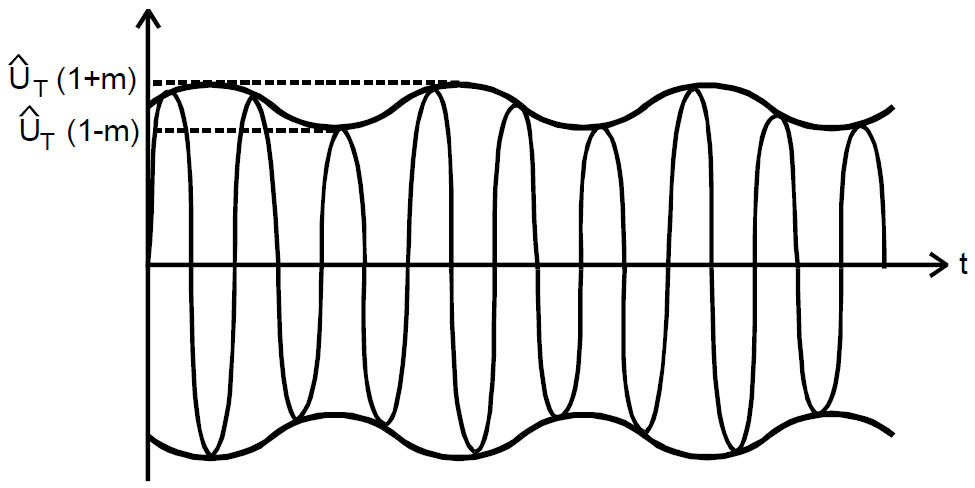
\includegraphics[width=14cm]{images/am-amplitude.png}
    \caption{Zeitabhängigkeit der Momentanspannung $U_\text{mod}(t)$ \cite{V59}.}
    \label{am:amplitude}
\end{figure}

Mithilfe trigonometrischer Umformulierung ergibt sich aus Gleichung \eqref{am:formel1} 
\begin{equation}
     U_\text{mod}(t) = U_\text{0,T} \left( \cos{\left(\omega_\text{T} t\right)} + \frac{m}{2}\cos{\left((\omega_\text{T} + \omega_\text{M}) t\right)} + \frac{m}{2}\cos{\left((\omega_\text{T} - \omega_\text{M}) t\right)}\right) \,. \label{am:formel2}
\end{equation}

Daraus ist zu erkennen, dass das Frequenzspektrum einer in dieser Art und Weise modelierten Schwingung aus 3 Linien mit den Kreisfrequenzen $\omega_\text{T} + \omega_\text{M}$, $\omega_\text{T} - \omega_\text{M}$ und $\omega_\text{T}$ besteht.
$\omega_\text{T}$ überträgt dabei keinerlei Informationen, da sie nicht von der Modulationsamplitude $U_\text{0,M}$ abhängt.
In der Praxis wird daher versucht diese zu unterdrücken, da sie mit einem unnötigen Energieverbrauch verbunden ist.
Die gesamte Information ist zudem bereits in einem Seitenband enthalten - bei mehreren Frequenzen in der Modulationsspannung verbreitern sich die äußeren Linien zu Frequenzbändern - und somit kann mithilfe eines geeigneten Bandpassfilters bereits im Modulationsprozess eine Seite unterdrückt werden.

Nachteile der Amplitudenmodulation sind die geringe Störsicherheit und die geringe Verzerrungsfreiheit.

\subsection{Frequenzmodulation}
\label{subsec:einstein}

Eine frequenzmodulierte Schwingung kann durch Gleichung
\begin{equation*}
    U(t) = U_\text{0} \sin{\left( \omega_\text{T} t + m \frac{\omega_\text{T}}{\omega_\text{M}} \cos{\left(\omega_\text{M} t\right)} \right)}
\end{equation*}
dargestellt werden.
Die Momentanfrequenz $f$ ergibt sich durch Ableiten des Arguments der Sinusfunktion zu
\begin{equation*}
    f(t) = \frac{\omega_\text{T}}{2 \pi} ( 1 - m \sin{\left(\omega_\text{M} t\right)}) \,.
\end{equation*}
Der Vorfaktor der Sinusfunktion $\frac{m \omega_\text{T}}{2 \pi}$ wird als Frequenzhub bezeichnet und gibt die Variationsbreite der Schwingungsfrequenz an.
Im folgenden soll nur der Fall der Schmalband-Frequenzmodulation (niedriger Frequenzhub) betrachtet werden, also 
\begin{equation*}
    m \frac{\omega_\text{T}}{\omega_\text{M}} \ll 1\,.
\end{equation*}
Ein Beispiel für eine frequenzmodulierte Schwingung ist in Abbildung \ref{fm:modulation} dargestellt.

\begin{figure}[!h]
    \centering
    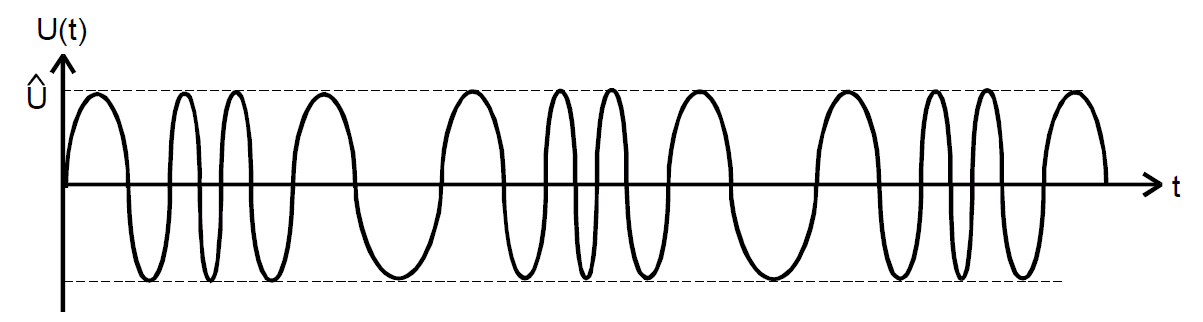
\includegraphics[width = 14cm]{images/fm-modulation.png}
    \caption{Zeitlicher Verlauf einer sinusförmig frequenzmodulierten Schwingung \cite{V59}.}
    \label{fm:modulation}
\end{figure}

Auch hier ist das Frequenzspektrum recht einfach was an der umgeformten Gleichung
\begin{equation*}
    U(t) = U_\text{0} \left( \sin{\left( \omega_\text{T} t \right) }\cos{\left(m\frac{\omega_\text{T}}{\omega_\text{M}} \cos{\left(\omega_\text{M} t\right)}\right)} + \cos{\left(\omega_\text{T} t\right)}\sin{\left(m\frac{\omega_\text{T}}{\omega_\text{M}} \cos{\left(\omega_\text{M} t\right)}\right)} \right)
\end{equation*}
zu erkennen ist.

Für eine schwach frequenzmodulierte Schwingung ergibt sich somit näherungsweise
\begin{equation}
    U(t) \approx U_\text{0} \left( \sin{\left(\omega_\text{T} t\right)} + \frac{m \omega_\text{T}}{2 \omega_\text{M}} \cos{\left((\omega_\text{T} + \omega_\text{M}) t\right)} + \frac{m \omega_\text{T}}{2 \omega_\text{M}} \cos{\left((\omega_\text{T} - \omega_\text{M}) t\right)}\right) \,, \label{fm:kleiner_hub}
\end{equation}
woraus sich wieder drei Teilschwingungen wie bei der amplitudenmodulierten Schwingung ergeben.
Der Unterschied liegt darin, dass die Trägerschwingung gegen die beiden Seitenlinien um $\frac{\pi}{2}$ verschoben ist.

\subsection{Modulationsschaltungen}
\label{subsec:debye}

\paragraph{Amplitudenmodulation}
Für die Amplitudenmodulation wird ein Gerät benötigt, welches das Produkt zweier Spannungen bildet.
Beispielsweise ist dafür eine Diode geeignet, prinzipiell kann jedoch jedes Bauelement verwendet werden, welches eine nicht-lineare Kennline besitzt.

\begin{figure}[!h]
    \centering
    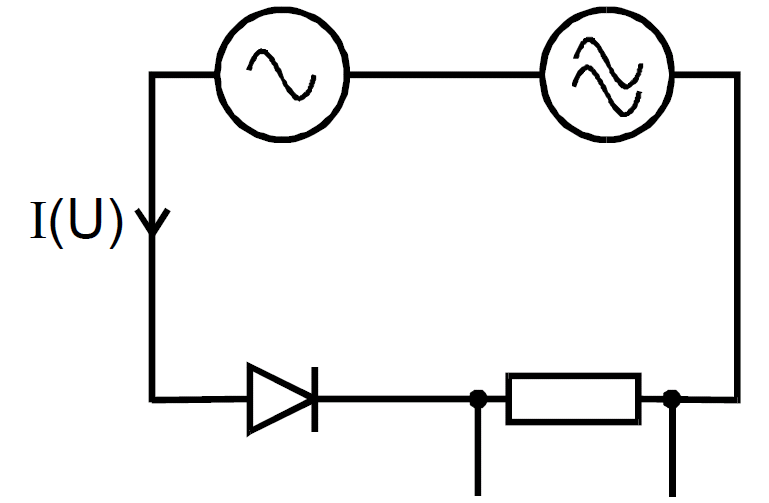
\includegraphics[width = 14cm]{images/modulationsschaltung.png}
    \caption{Primitive Modulationsschaltung \cite{V59}.}
    \label{modulationsschaltung_einfach}
\end{figure}

Betrachtet man die Potenzreihenentwicklung der Diodenkennline einer primitiven Modulationsschaltung nach Abbildung \ref{modulationsschaltung_einfach}
\begin{equation*}
    I = a_0 + a_1 U + a_2 U^2 + \dots
\end{equation*}
und setzt die Summe aus Träger- und Modulationsspannung ein
\begin{equation*}
    I ( U_\text{T} + U_\text{M} ) = a_0 + a_1 ( U_\text{T} + U_\text{M} ) + a_2 ( U_\text{T}^2 + U_\text{M}^2 ) + 2 a_2 U_\text{T} U_\text{M} + \dots \,,
\end{equation*}
so ist zu erkennen, dass neben dem gewünschten Glied $U_\text{T} U_\text{M}$ auch störende Terme auftreten.
Deren Frequenzen liegen jedoch weit außerhalb des zu übertragenden Frequenzbereichs, sodass der Einsatz eines Bandpassfilters diese unterdrückt.

Eine alternative Schaltung, welche diese störenden Terme gar nicht erst erzeugt, ist der sogenannte Ringmodulator nach Abbildung \ref{am:ringmodulator}.

\begin{figure}[!h]
    \centering
    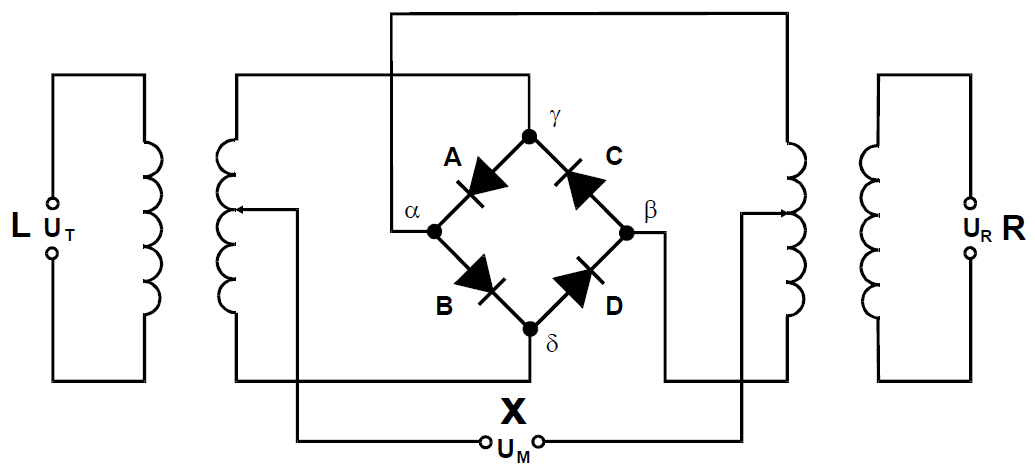
\includegraphics[width = 14cm]{images/ringmodulator.png}
    \caption{Schaltbild eines Ringmodulators \cite{V59}.}
    \label{am:ringmodulator}
\end{figure}

Die Diodenzweige A und B sowie C und D stellen je einen Spannungsteiler für die Trägerspannung $U_\text{T}$ dar, welche über den Eingang L eingespeist wird.
An den Punkten $\alpha$ und $\beta$ werden die Spannungen abgegriffen und über einen Hochfrequenz-Transformator an den Ausgang R gegeben.
Wird keine Modulationsspannung angelegt, so bleibt das Teilungsverhältnis der Diodenzweige konstant und es ist keine Spannung abzugreifen.
Mit einer Modulationsspannung $U_\text{M}$ jedoch ändern sich die Verhältnisse im Rhythmus von $U_\text{M}(t)$.
Bei idealen Verhältnissen gilt
\begin{equation*}
    U_\text{R}(t) = \gamma U_\text{T}(t) U_\text{M}(t)
\end{equation*}
mit $\gamma$ als Propotionalitätskonstante mit der Maßeinheit $\si{1\per\volt}$ und es liegt somit keine Trägerabstrahlung vor.
Mit den Ansätzen für die Spannungen mit 
\begin{eqnarray*}
    U_\text{T}(t) &=& \hat{U}_\text{T} \cos{\left(\omega_\text{T} t\right)} \\
    U_\text{M}(t) &=& \hat{U}_\text{M} \cos{\left(\omega_\text{M} t + \varphi \right)}
\end{eqnarray*}
ergibt sich
\begin{equation*}
    U_\text{R}(t) = \gamma \hat{U}_\text{T} \hat{U}_\text{M} \frac{1}{2} \left( \cos{\left( \left( \omega_\text{T} + \omega_\text{M} \right) t + \varphi \right)} + \cos{\left( \left( \omega_\text{T} - \omega_\text{M} \right) t - \varphi \right)} \right) \,.
\end{equation*}
Es treten also nur die Seitenlinien auf.

\paragraph{Frequenzmodulation}
Wir betrachten ein Schaltungsbeispiel für einen Frequenzmodulator mit geringem Frequenzhub, sodass Gleichung \eqref{fm:kleiner_hub} ihre Gültigkeit hat (Abb.\ref{fig:fm-erzeugung}).
Da bei einem Ringmodulator nur die beiden Seitenbänder auftreten, ist es möglich durch addieren einer um $90^\circ$ in der Phase verschobenen Trägerspannung $U_\text{T}$ an den Ausgang R eine Frequenzmodulation zu erzeugen.

\begin{figure}[!h]
    \centering
    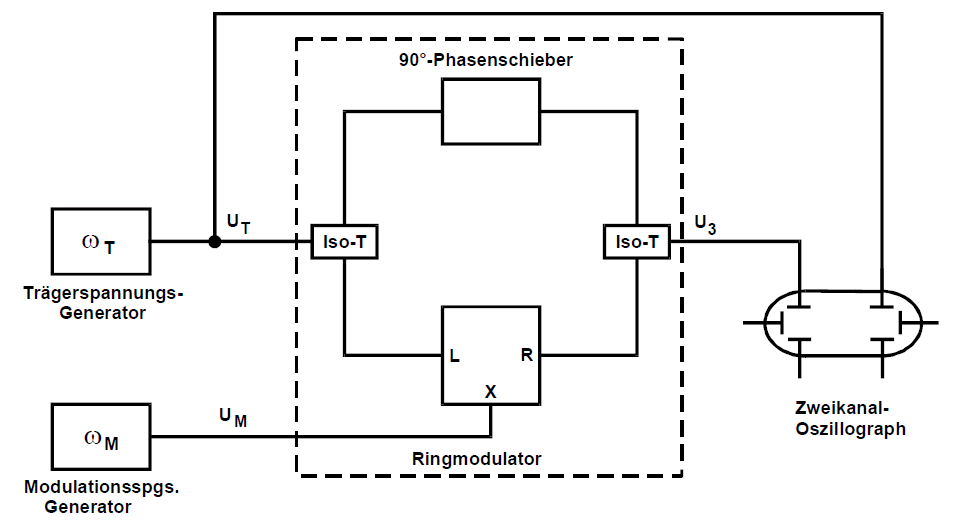
\includegraphics[width = 14cm]{images/fm_schaltbild.png}
    \caption{Schaltbild für einen Frequenzmodulator mit einem geringen Frequenzhub \cite{V59}.}
    \label{fig:fm-erzeugung}
\end{figure}

\subsection{Demodulator - Schaltungen}
\label{subsec:debye}

\paragraph{Demodulation amplitudenmodulierter Schwingungen}
Zur Demodulation lässt sich auch hier ein Ringmodulator verwenden.
Das modulierte Signal wird auf den Eingang R gegeben und besteht bekannterweise aus den Frequenzen $\omega_\text{T}$, $\omega_\text{T} - \omega_\text{M}$ und $\omega_\text{T} + \omega_\text{M}$.
Wird nun auf den Eingang L eine Spannung mit der Frequenz $\omega_\text{T}$ gelegt, so erhält man am Ausgang X eine Spannung mit den Frequenzen $\omega_\text{M}$, $2\omega_\text{T} - \omega_\text{M}$ und $2\omega_\text{T} + \omega_\text{M}$.
Da $\omega_\text{T}$ meist sehr viel größer ist als $\omega_{M}$, bleibt nach verwenden eines Tiefpassfilters nur noch die gewünschte Spannung mit der Modulationsfrequenz $\omega_\text{M}$ übrig.
In der Praxis ist es nötig Phasenregelkreise zu verwenden, um eine phasenstarre Trägerfrequenz $U_\text{T}$ zu erzeugen.
In Abbildung \ref{fig:adm_ringmodulator} ist das Schaltbild einer solchen Schaltung dargestellt.

\begin{figure}[!h]
    \centering
    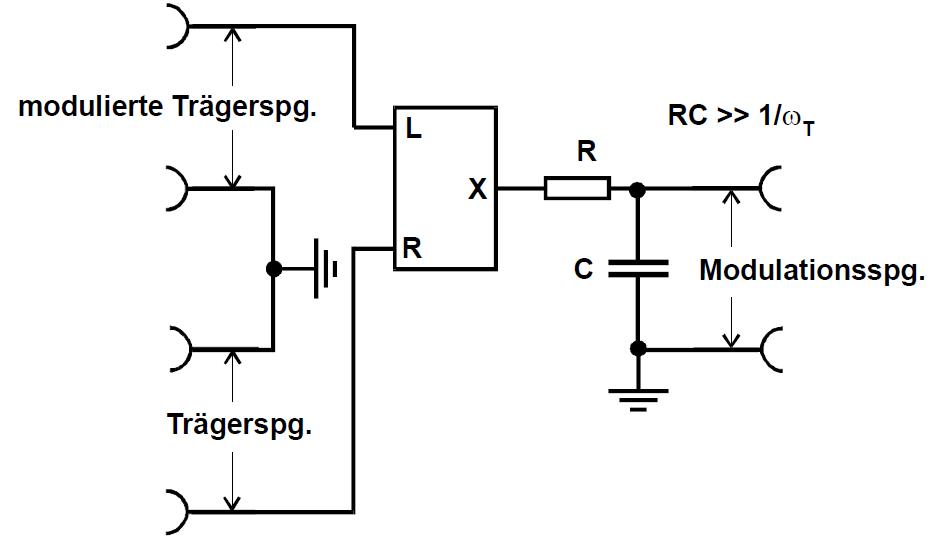
\includegraphics[width = 14cm]{images/adm_ringmodulator.png}
    \caption{Demodulator-Schaltung mit einem Ringmodulator \cite{V59}.}
    \label{fig:adm_ringmodulator}
\end{figure}

Um das Problem einer festen Phasenbeziehung zwischen der Signal- und der Referenzspannung zu vermeiden, kann eine Demodulatorschaltung nach Abbildung \ref{fig:dioden-schaltung} verwendet werden.

\begin{figure}[!h]
    \centering
    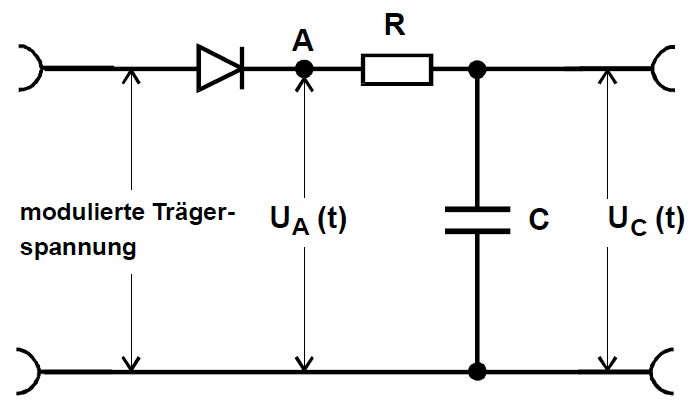
\includegraphics[width = 14cm]{images/adm_diode.png}
    \caption{Demodulator-Schaltung mit einer Diode \cite{V59}.}
    \label{fig:dioden-schaltung}
\end{figure}

Die Diode schneidet alle negativen Halbwellen ab, sodass eine Spannung übrig bleibt, welche in Abbildung \ref{adm:spannung} dargestellt ist.

\begin{figure}[!h]
    \centering
    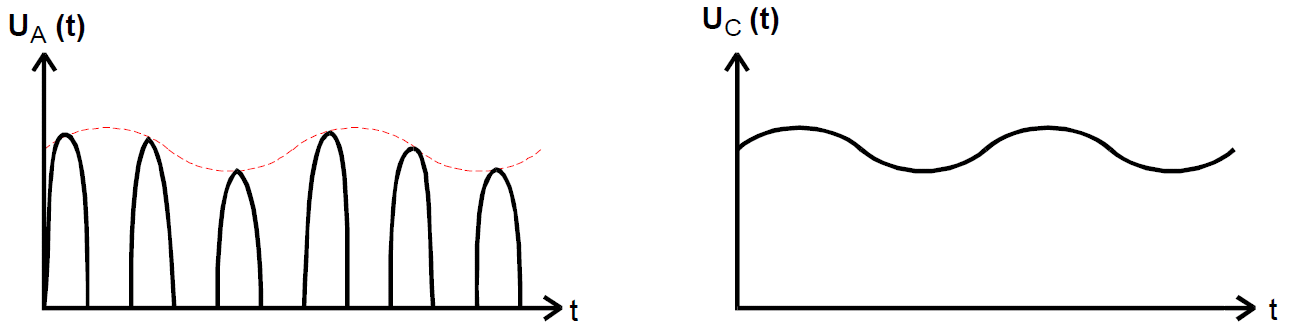
\includegraphics[width = 14cm]{images/adm_spannung.png}
    \caption{\textbf{links:} Gleichgerichtete modulierte Hochfrequenz-Spannung. \textbf{rechts:} Ausgangsspannung hinter dem Tiefpass \cite{V59}.}
    \label{adm:spannung}
\end{figure}

Für einen geringen Modulationsgrad kann die in der Realität exponentiell verlaufende Diodenkennlinie als linear angesehen werden, sodass sich am Ausgang direkt die Modulationsspannung ablesen lässt.

\paragraph{Demodulation frequenzmodulierter Schwingungen}
Ein Flankenmodulator ist ein Beispiel für eine Demodulationsschaltung für frequenzmodulierte Signale.
Dieser besteht aus einem einfachen Schwingkreis, bei dem die Frequenzabhängigkeit der Kondensatorspannung im Falle erzwungener Schwingungen ausgenutzt wird (Abb. \ref{fdm:schaltung}).

\begin{figure}[!h]
    \centering
    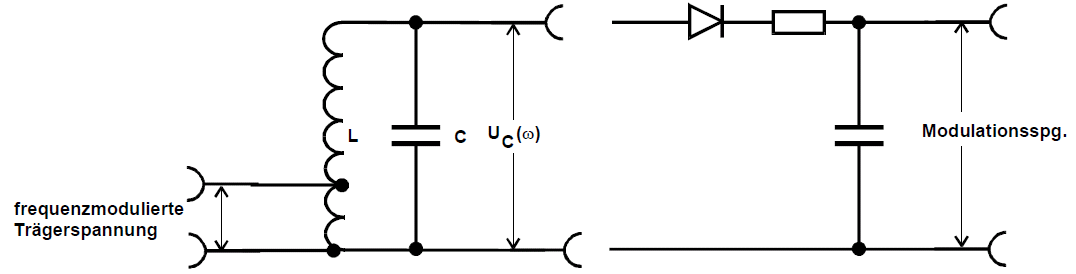
\includegraphics[width = 14cm]{images/fdm_schaltung.png}
    \caption{Beispiel einer Demodulatorschaltung für frequenzmodulierte Schwingungen \cite{V59}.}
    \label{fdm:schaltung}
\end{figure}

Die Resonanzfrequenz des Schwingkreises wird dabei so eingestellt, dass die Trägerfrequenz $\omega_\text{T}$ mitten in der steilen Flanke der Resonanzkurve liegt (Abb. \ref{fdm:resonanz}).

\begin{figure}[!h]
    \centering
    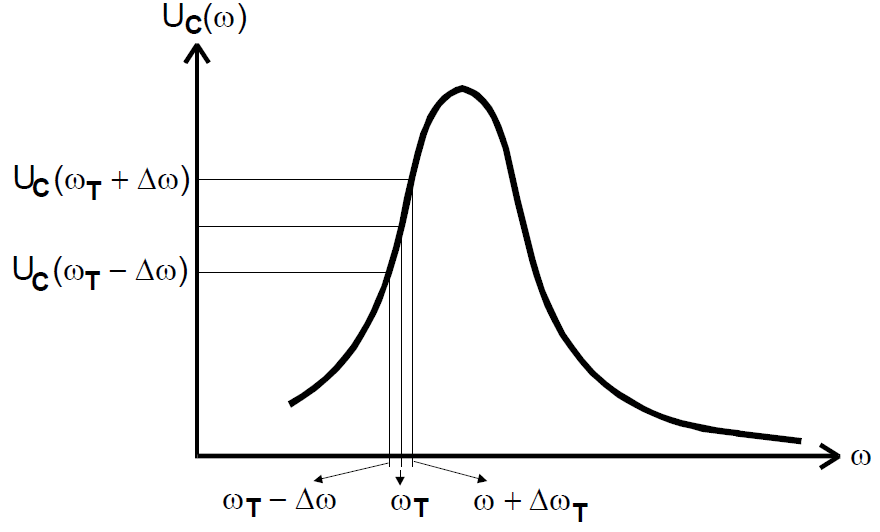
\includegraphics[width = 14cm]{images/fdm_resonanz.png}
    \caption{Resonanzkurve des Schwingkreises im Flankenmodulator \cite{V59}.}
    \label{fdm:resonanz}
\end{figure}

Dieses Verfahren überführt die Frequenzmodulation in eine Amplitudenmodulation, indem eine hochfrequente Spannung am Ausgang erzeugt wird, deren Amplitude im Rhythmus der Modulation schwankt.
Diese kann durch das zuvor beschriebene Verfahren demoduliert werden.
Eine besonders unverzerrte Demodulation erhält man, wenn man den Frequenzhub möglichst klein wählt.
Zudem kann durch eine Gegentaktschaltung eine verbesserte Linearität der Demodulations-Kennlinie erreicht werden.

\section{Durchführung}
\label{sec:durchführung}

\paragraph{a)}
Mithilfe eines Ringmodulators soll eine amplitudenmodulierte Schwingung mit Trägerunterdrückung erzeugt werden.
Die dabei entstehende Schwebung soll mithilfe eines Oszilloskops visualisiert werden.

\paragraph{b)}
Unter Zuhilfenahme eines Frequenzanalysators wird das Frequenzspektrum der amplitudenmodulierten Schwingung untersucht.
Der Modulationsgrad $m$ kann daraus bestimmt werden.

\paragraph{c)}
Analog zu Aufgabenteil a und b wird nun eine Diode zur Modulation verwendet.
Es werden dieselben Eigenschaften untersucht, doch wird insbesondere gezeigt, dass auch Oberwellen von $\omega_\text{T}$ auftreten.

\paragraph{d)}
\label{par:d_}
Zur Demodulation einer modulierten Schwingung wird ein Ringmodulator verwendet.
Mithilfe einer Schaltung nach Abbildung \ref{fig:am-schaltung-demodulation} wird zunächst die Proportionalität der anliegenden Gleichspannung am Ausgang X mit dem Cosinus der Phase $\varphi$ zwischen den beiden Eingängen R und L gezeigt.
Dazu wird die Schaltung nach Abbildung \ref{fig:am-schaltung-demodulation} verwendet.

\begin{figure}[!h]
    \centering
    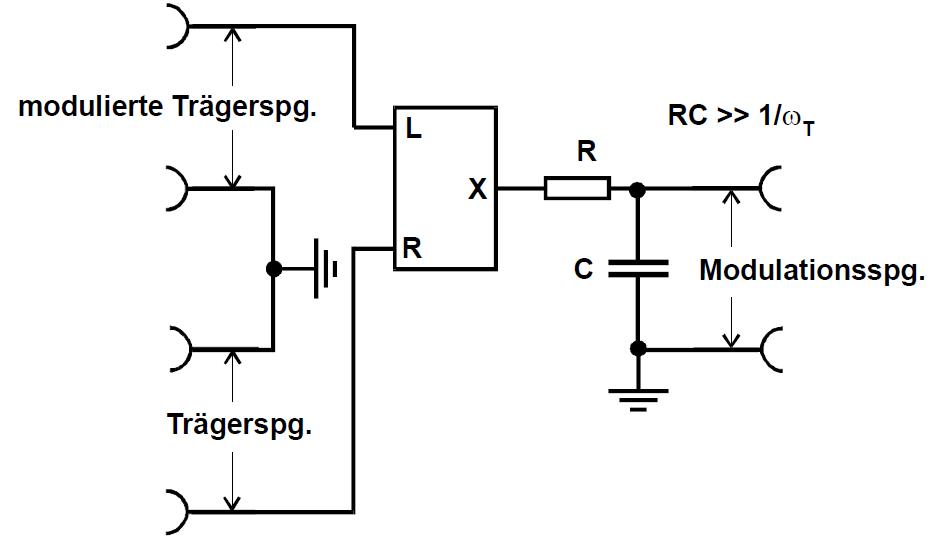
\includegraphics[width = 14cm]{images/adm_ringmodulator.png}
    \caption{Demodulator-Schaltung mit einem Ringmodulator \cite{V59}.}
    \label{fig:am-schaltung-demodulation}
\end{figure}

\paragraph{e)} 
\label{par:e_}
Statt eines Spannungsmessgeräts wird ein Oszillograph an den Ausgang X des Ringmodulators angeschlossen, sodass es möglich ist die Modulationsspannung praktisch unverzehrt zurückzuerhalten.

\paragraph{f)} % (fold)
\label{par:g}
Mithilfe einer Gleichrichterdiode wird eine amplitudenmodulierte Schwingung demoduliert.
Dabei wird die Zeitabhängigkeit vor dem Tiefpass und hinter dem Tiefpass dargestellt.

\paragraph{g)} % (fold)
\label{par:g_}
Es soll eine frequenzmodulierte Schwingung erzeugt werden und die Zeitabhängigkeit der modulierten Schwingung auf dem Schirm des Oszillographen dargestellt werden.
Aus dem erzeugten Bild lässt sich der Frequenzhub und der Modulationsgrad ermitteln.
Zudem soll das Frequenzspektrum untersucht werden.

\paragraph{h)} % (fold)
\label{par:h_}
Im letzten Abschnitt wird eine frequenzmodulierte Spannung demoduliert und das Ergebnis auf den Oszillographen gegeben.
